\documentclass[12pt]{article}
\linespread{1.15}
\usepackage[margin=1in]{geometry}
\usepackage{graphicx,longtable,array,url}
\setlength{\parskip}{4pt}
\title{\textbf{A Byte-Locked Structural and Mutational Atlas of the Oropouche Virus Replication Machinery:\\Outbreak-Era Substitutions in L, N, and Gn/Gc Mapped onto Experimental and Homolog-Anchored Structures}}
\author{Open-Data Biocomputation Research Program, Project 2 (oropouche-structure)}
\date{September 23, 2026}
\begin{document}
\maketitle
\tableofcontents
\vspace{1em}
\begin{abstract}
Oropouche virus (OROV), a tripartite negative-sense RNA orthobunyavirus (Peribunyaviridae), caused the largest recorded outbreak in its history across South America in 2023--2025, driven by a novel reassortant lineage (BR2015-2024). Experimental structural coverage of OROV remains limited to a single crystal structure, the Gc glycoprotein head domain (PDB 6H3X), and no systematic, quality-tracked structural atlas or reproducible outbreak-versus-historical substitution catalog exists. Here we byte-locked 791 complete OROV segment sequences (126 L, 265 M, 400 S; sampling years 1955--2025) from NCBI GenBank with SHA-256 manifests, locked success gates and three positive-control validations in writing before examining any outcome data, and derived a reference-anchored amino-acid substitution catalog contrasting outbreak-era (2022+) with historical (pre-2020) proteins. All three positive controls passed: canonical bunyavirus RdRp motifs were recovered in 126/126 L proteins; the pipeline reproduced the known N-glycan sequon and alignment of the experimental 6H3X Gc head construct (98.6\% identity); and a five-substitution spike-in was recovered exactly with zero false positives. The resulting catalog is byte-identical on re-run and contains 36 substitutions at historically conserved columns (L 28, M 6, N 2), including a near-fixed Gc substitution I1203T (97.3\% of outbreak sequences), a seven-site cluster in the L polymerase core, and two N substitutions, one of which (M170T) maps 8.1 \AA{} from the RNA phosphate backbone in the Schmallenberg virus N--RNA complex (71.1\% identity anchor). Single-sequence ESMFold models failed our structural positive control (17.7 \AA{} global CA RMSD against 6H3X; mean pLDDT 0.38--0.61), so we report that negative result in full and restrict all structural claims to experimental and homolog-anchored evidence with per-residue confidence marking. This is, to our knowledge, the first byte-locked, validation-gated substitution-and-structure resource for OROV, and it nominates Gc I1203T and the L polymerase-core cluster as priority candidates for experimental follow-up.
\end{abstract}

\section{Introduction}
Oropouche virus (OROV) is an enveloped orthobunyavirus with a tri-segmented, single-stranded, negative-sense RNA genome. The small (S) segment encodes the nucleoprotein N and the non-structural interferon antagonist NSs; the medium (M) segment encodes a polyprotein cleaved into the glycoproteins Gn and Gc and the NSm protein; the large (L) segment encodes the RNA-dependent RNA polymerase (RdRp), a multifunctional cap-snatching polymerase of roughly 2,200 amino acids. OROV is transmitted primarily by \textit{Culicoides paraensis} midges and has caused recurrent outbreaks in South and Central America since 1955.

Beginning in late 2023, OROV caused its largest documented outbreak, with more than 6,300 laboratory-confirmed cases in the Brazilian western Amazon between 2022 and 2024 and subsequent spread to previously non-endemic Brazilian states, other South American countries, and travel-associated cases in Cuba, Europe, and the United States. Nascimento, Giovanetti and colleagues (Nature Medicine 2024) sequenced 382 outbreak genomes and showed that the upsurge coincides with a novel reassortant lineage, BR2015-2024, combining an M segment of eastern-Amazon ancestry (2009--2018) with L and S segments of Peru--Colombia--Ecuador ancestry (2008--2021). Their work established the phylogenetic and phylodynamic picture but did not produce an amino-acid-level substitution catalog contrasting outbreak and historical proteins, nor any structural analysis.

Structural knowledge of OROV is thin. The only experimental structure of any OROV protein is the crystal structure of the Gc head domain (PDB 6H3X, 221 modeled residues), deposited by Hellert and colleagues in 2018. No experimental structures exist for the L polymerase, the N protein, Gn, or full-length Gc. A 2025 bioinformatic study (``Charting the Proteins of Oropouche Virus,'' \textit{Viruses} 17:1434) built single-sequence AlphaFold2/Phyre2 models of the major proteins and predicted epitopes, but did not track per-residue confidence against any outbreak diversity, did not validate against 6H3X, and did not analyze mutations. Homolog structures from related peribunyaviruses are available: the La Crosse virus (LACV) full-length L protein (PDB 6Z6B) and its N-terminal endonuclease domain (PDB 2XI7), and the Schmallenberg virus (SBV) nucleoprotein--RNA complex (PDB 4JNG).

This study was designed around three properties that prior OROV computational work lacks. First, byte-level reproducibility: every input sequence is locked with a SHA-256 checksum in a manifest, and the full analysis re-runs to byte-identical outputs. Second, pre-registered validation: success gates and three positive controls were locked in writing before any outbreak-versus-historical contrast was examined, and negative results are preserved rather than re-fished. Third, honest structural confidence: every structural claim is tied either to experimental coordinates or to explicitly labeled homology anchors, and a failed structure-prediction positive control is reported as such.

\section{Hypothesis and locked gates}
\textbf{Hypothesis.} The 2022--2025 outbreak lineage carries a definable set of amino-acid substitutions, relative to historically conserved residues, in the replication machinery (L RdRp, N) and entry machinery (Gn/Gc); a subset of these substitutions occupies structurally interpretable positions near functional centers (polymerase core, endonuclease active site, RNA-binding surface, glycan sites).

\textbf{Locked gates} (written 2026-09-23 13:30 IST, before outcome data were examined; full text in \texttt{GATES\_LOCKED.md}, committed to the repository as a standalone commit preceding all results commits):
\begin{itemize}
\item \textbf{G1 (data).} $\geq$50 complete L-segment sequences byte-locked with SHA-256 checksums; M and S sets locked alongside; manifest records accessions, per-record checksums, timestamps, and sources.
\item \textbf{G2 (structure).} Structural models only from real sources; per-residue pLDDT tracked; residues with pLDDT $<$70 marked THIN on every figure and in every claim; no claim rests on thin regions. Structural positive control: the modeling/scoring pipeline must recover the known architecture of PDB 6H3X and the canonical L motifs.
\item \textbf{G3 (mutation map).} The outbreak-versus-historical substitution list must be byte-identical on re-run from the manifest, reported with counts, frequencies, and segment-lineage context.
\item \textbf{G4 (validation before novel claims).} PC1: motif scanner recovers canonical RdRp motifs (including motif C ``SDD'') in 100\% of complete L ORFs. PC2: the pipeline recovers the known N-glycan sequon of PDB 6H3X in the reference M polyprotein. PC3: a five-substitution engineered spike-in is recovered exactly. All three must pass before any outbreak result is read.
\end{itemize}
Era definitions were locked: outbreak $=$ sampled 2022-01-01 or later; historical $=$ sampled before 2020-01-01; 2020--2021 and undated records form an excluded buffer.

\section{Data and Methods}
\subsection{Data acquisition and byte-lock}
All sequences were fetched from NCBI GenBank via E-utilities on 2026-09-23. Segment-specific queries used organism filter \texttt{Oropouche virus[Organism]} with sequence-length windows (L: 6000--8000 nt; M: 3800--5200 nt; S: 650--1300 nt), and records were retained when the title indicated a complete segment and segment identity keywords matched. Sampling year, country, and host were parsed from GenBank structured metadata. Nucleotide sets were written to FASTA and locked with SHA-256 checksums; a 791-row manifest records accession, segment, length, year, era, country, host, per-record SHA-256, and title. Protein sequences were extracted from GenBank CDS annotations (not de-novo ORF prediction); records lacking a full-length annotated polyprotein CDS were counted as missing rather than guessed (3 of 265 M records).

\subsection{Reference-anchored substitution calling}
For each protein set, a reference was chosen deterministically (modal length among historical sequences, lowest accession on ties; for M the mat-peptide-annotated reference KC759123.1 was used). Every historical sequence was aligned to the reference (parasail striped Needleman--Wunsch, BLOSUM62, gap open 10, extend 1), and per-column historical majorities and fractions were computed. A column was called conserved when the historical majority fraction was $\geq$0.9 with $\geq$20 aligned sequences. Each outbreak sequence was then aligned and substitutions were called at conserved columns where the outbreak residue differed from the historical majority; substitutions were retained in the catalog at outbreak frequency $\geq$0.05 and count $\geq$3. M-polyprotein regions were locked as Gn 1--350, NSm 351--481, Gc 482--1420 (literature annotation corroborated by the 6H3X construct mapping, which begins at reference residue 482). L domains were locked as endonuclease 1--185 (LACV 2XI7 homology), polymerase core $\pm$400 residues around motif C, remainder other.

\subsection{Positive controls}
PC1 scanned all complete L proteins for motif C (SDD) and premotif A (DxxKW). PC2 aligned the 6H3X construct sequence to the reference M polyprotein and checked that its single N-glycan sequon maps to the identical triplet. PC3 inserted five engineered substitutions into a copy of the L reference at historically conserved columns and required the caller to return exactly the baseline (reference-versus-majority) call set plus the engineered five, with zero false positives and zero misses. PC3 failed on its first run, exposing that the reference itself carries minority alleles at nine conserved columns; the control was corrected to a baseline-relative expectation and the failure and fix were logged per protocol.

\subsection{Structure prediction, validation, and homolog anchoring}
Outbreak-consensus sequences were built per protein (outbreak majority per reference column, requiring $\geq$10 covering sequences). Four targets were folded with the ESMFold API (single-sequence ESM-2 language model): N full-length (231 aa), Gn (350 aa), Gc head (222 aa), and the L endonuclease domain (185 aa); per-residue pLDDT was read from CA B-factors (0--1 scale, verified against a ubiquitin control, mean 0.91). The structural positive control folded the exact 6H3X construct sequence and superposed it on experimental 6H3X coordinates using sequence-identical CA pairs (Bio.PDB SVD superposition), with additional 30-residue sliding-window RMSD to assess local topology. Homolog anchoring aligned OROV sequences to experimental homologs---LACV endonuclease 2XI7 (with catalytic Mn$^{2+}$ ions and the inhibitor DPBA) and SBV N--RNA complex 4JNG---and transferred substitution positions through alignment columns, reporting alignment identity and minimum distances to functional centers (Mn ions; RNA phosphate backbone).

\section{Results}
\subsection{Dataset}
The byte-locked dataset comprises 791 unique complete-segment records (zero duplicate sequences): 126 L, 265 M, and 400 S segments sampled from 1955 to 2025 (Figure 1). Era composition: L 69 historical / 52 outbreak / 5 buffer; M 69 / 191 / 5 (262 with extractable full polyprotein CDS); S-derived N 135 / 208 / 57. The L gate of $\geq$50 complete segments was cleared 2.4-fold.

\subsection{All validation gates passed before outcome data were read}
PC1: motif C (SDD) and premotif A (DxxKW) were present in 126/126 complete L proteins (length range 2167--2252 aa). PC2: the 6H3X construct aligned to the reference M polyprotein at 98.6\% identity over 222 residues (reference span 482--703), and its single N-glycan sequon (NIT) mapped to the identical NIT triplet at reference position 676. PC3: after the logged first-run failure and control correction, the caller recovered 5/5 engineered substitutions exactly with zero false positives. G3: the full pipeline re-run produced a byte-identical substitution table (diff-verified).

\subsection{The outbreak-versus-historical substitution catalog}
The catalog contains 36 substitutions at historically conserved columns: 28 in L, 6 in M, 2 in N (Figure 3; full table in Appendix A). Headline features:
\begin{itemize}
\item \textbf{Gc I1203T is near-fixed in the outbreak}: 183/188 outbreak M sequences (97.3\%) at a position conserved at 100\% across 69 historical sequences. This is the single most differentiated position in the entire proteome-wide contrast.
\item \textbf{An L polymerase-core cluster}: seven positions in a 70-residue window (787--856, reference KP026179.1 numbering) each carried by $\sim$60\% of outbreak L sequences (K787N, Q788R, V790L, N791S, I799L, N802E, K850R, N855M, D856M), plus T853L/Q at lower frequency, and L1114V at 80.8\%.
\item \textbf{L lineage markers at high frequency}: T201A (90.4\%), V338I (86.5\%), A565T (88.5\%), S677A (78.8\%), I2187V (78.8\%); endonuclease-domain substitutions R27P (11.8\%) and A68T (31.4\%).
\item \textbf{N protein}: M170T (36.5\%) and N133K (15.9\%).
\item \textbf{Gn}: A68T (23.9\%) and V176I (21.8\%); Gc also carries A552S (18.6\%), I957V (20.7\%), P1325T (7.4\%).
\end{itemize}

\subsection{Structural analysis: a preserved negative result for single-sequence folding}
ESMFold single-sequence models of all four targets returned uniformly low confidence (mean pLDDT 0.38--0.61 on the 0--1 scale; Figure 6). The structural positive control adjudicated whether the models could nonetheless support claims: the ESMFold model of the exact 6H3X construct superposed on the experimental structure with a global CA RMSD of 17.7 \AA{} over 221 sequence-identical pairs---the global fold was \textbf{not} recovered (Figure 4A). Sliding-window analysis showed local topology is partially recovered (6 of 20 thirty-residue windows below 3 \AA{}; Figure 4B), but per gate G2 no structural claim may rest on these models. We therefore report the ESMFold atlas as a negative result: for these OROV targets, single-sequence language-model folding is not a substitute for MSA-based prediction or experiment. This is consistent with the models' own pLDDT and with the paucity of close OROV structural templates, and it preserves the finding for others rather than re-fishing until a plausible-looking model appears.

\subsection{Homolog-anchored structural context for the substitution sites}
All structural interpretation was instead anchored to experimental coordinates (Figure 5).
\textbf{Gc head (experimental, 6H3X).} The outbreak substitution A552S lies inside the crystallized head domain (residues 482--702). Residue 552 sits in a moderately packed environment (18 CA neighbors within 10 \AA{}) and 19.4 \AA{} from the N-glycan sequon at 676; an Ala-to-Ser exchange introduces a polar side chain at a packed position in the head domain of the fusion protein. The near-fixed I1203T and the lower-frequency I957V and P1325T lie outside the crystallized construct (Gc stem/anchor regions) and are marked as structurally uninterpreted.
\textbf{L endonuclease (homolog, 2XI7).} The OROV L endonuclease domain aligns to the LACV endonuclease crystal structure at 40.3\% identity over 181 columns, comfortably within homology-transfer range for fold annotation. Neither outbreak substitution maps into the catalytic shell (residues 34, 52, 79, 92, 93 within 4 \AA{} of the two Mn$^{2+}$ ions): R27P maps 13.8 \AA{} and A68T 25.4 \AA{} from the nearest Mn ion.
\textbf{L polymerase core.} The 787--856 cluster flanks the canonical polymerase motifs (motif C SDD present in all sequences); the affected positions sit within the core region but cannot be placed on OROV-specific coordinates, so they are reported as sequence-level findings anchored to the LACV full-length L fold family (6Z6B) without per-residue structural claims.
\textbf{N protein (homolog, 4JNG).} OROV N aligns to the SBV nucleoprotein at 71.1\% identity over 225 columns. M170T maps to a position whose closest approach to the RNA phosphate backbone in the N--RNA complex is 8.1 \AA{} (any atom), at the RNA-binding surface; N133K maps 15.9 \AA{} away, not RNA-proximal. M170T is thus the one outbreak substitution in N with a direct structural hypothesis: modulation of RNA binding in the ribonucleoprotein complex.

\section{Discussion}
Three contributions stand out. First, the resource itself: 791 byte-locked complete segments with per-record checksums, a validation-gated pipeline whose every claim is reproducible from the manifest, and a substitution catalog that re-runs byte-identically. To our knowledge no prior OROV study---genomic or structural---meets this bar, and the manifest plus code allow any group to extend the catalog as new genomes appear.

Second, the mutation map nominates concrete experimental targets. Gc I1203T, near-fixed (97.3\%) in the outbreak at a historically invariant position, is the standout: Gc is the class-II fusion protein mediating entry, and position 1203 lies in the membrane-proximal stem/anchor region that rearranges during fusion. The seven-site L polymerase-core cluster at $\sim$60\% frequency is the second priority: polymerase-core substitutions in other segmented negative-strand viruses modulate replication kinetics and host range. N M170T, 8.1 \AA{} from the RNA backbone in the homolog complex, is the third.

Third, the interpretation must be disciplined about what these frequencies mean. The outbreak is dominated by the BR2015-2024 reassortant, whose L and S segments descend from a Peru--Colombia--Ecuador lineage distinct from the eastern-Amazon historical majority. A high outbreak frequency at a historically conserved column is therefore primarily a \emph{lineage marker} of the reassortant's ancestry, not direct evidence of adaptation during the 2022--2025 transmission surge. The catalog cannot by itself distinguish ancestry from selection; it can and does nominate the positions where that distinction is worth experimentally testing. We report both the counts and this caveat rather than overclaiming adaptation.

The structural negative result deserves emphasis. Single-sequence ESMFold failed the 6H3X positive control by a wide margin (17.7 \AA{} global RMSD), despite returning plausible-looking ribbons. Had we followed the common practice of publishing unvalidated predicted models, every downstream ``structural interpretation'' would have rested on a wrong fold. The honest output is: (i) experimental Gc head coordinates carry the A552S analysis; (ii) homolog anchors at 40--71\% identity carry the L-endonuclease and N analyses, explicitly labeled; (iii) everything else is marked thin or uninterpreted. MSA-based folding (ColabFold-scale) of the outbreak consensus L, N, and Gn/Gc remains the clear next step, and the byte-locked targets are provided for exactly that.

\section{Limitations}
(1) Reference-anchored calling measures differences against historical majorities, not ancestral reconstructions; lineage-versus-adaptation is unresolved as discussed. (2) Historical sampling is geographically and temporally uneven (69--135 sequences over 65 years), so ``historically conserved'' is sampling-dependent; we mitigated with $\geq$20-coverage and $\geq$0.9-fraction thresholds. (3) No MSA-based structure prediction was possible in the compute envelope; structural interpretation beyond 6H3X is homology-labeled. (4) NSs was excluded from the catalog after a CDS-annotation parsing gap (only 1/400 S records yielded a product-named NSs CDS); the S-segment analysis covers N only. (5) Buffer-era (2020--2021) and undated records were excluded by design.

\section{Conclusions}
A byte-locked, validation-gated atlas of OROV replication and entry proteins yields 36 outbreak-lineage substitutions at historically conserved positions, nominates Gc I1203T, an L polymerase-core cluster, and N M170T for experimental follow-up, and demonstrates---by preserved negative result---that single-sequence structure prediction is not yet a valid substitute for experimental or MSA-based structures in this system.

\section*{Data and code availability}
Repository: \url{https://github.com/uditakankananonononono/oropouche-structure} (slice \texttt{oropouche/}): locked gates, fetch and analysis code, manifests with SHA-256 checksums, substitution table, validation outputs, figures, and this paper. Bulk nucleotide sets are re-derivable from the manifest accession list; checksums verify identity.

\begin{thebibliography}{9}
\small
\bibitem{natmed} Nascimento V.A.D., Giovanetti M., et al. Human outbreaks of a novel reassortant Oropouche virus in the Brazilian Amazon region. \textit{Nature Medicine} (2024). \url{https://www.nature.com/articles/s41591-024-03300-3}
\bibitem{h3x} Hellert J., Aebischer A., Wernike K., Haouz A., Brocchi E., Reiche S., Guardado-Calvo P., Beer M., Rey F.A. Oropouche Virus Glycoprotein Gc Head Domain. PDB 6H3X (2019). \url{https://www.rcsb.org/structure/6H3X}
\bibitem{reguera} Reguera J., Weber F., Cusack S. Bunyaviridae RNA polymerases (L-protein) have an N-terminal, influenza-like endonuclease domain, essential for viral cap-dependent transcription. \textit{PLoS Pathogens} 6(9):e1001101 (2010). PDB 2XI7. \url{https://www.rcsb.org/structure/2XI7}
\bibitem{z6b} Structure of full-length La Crosse virus L protein (polymerase). PDB 6Z6B. \url{https://www.rcsb.org/structure/6Z6B}
\bibitem{jng} Schmallenberg virus nucleoprotein-RNA complex. PDB 4JNG. \url{https://www.rcsb.org/structure/4JNG}
\bibitem{charting} Charting the Proteins of Oropouche Virus. \textit{Viruses} 17(11):1434 (2025). \url{https://doi.org/10.3390/v17111434}
\bibitem{ceara} Molecular Epidemiology of Oropouche Virus, Cear\'a State, Brazil, 2024. \textit{Emerging Infectious Diseases} 31(4):24-1471 (2025).
\bibitem{esm} Lin Z., et al. Evolutionary-scale prediction of atomic-level protein structure with a language model. \textit{Science} 379:1123--1130 (2023).
\bibitem{af} Jumper J., et al. Highly accurate protein structure prediction with AlphaFold. \textit{Nature} 596:583--589 (2021).
\end{thebibliography}

\clearpage
\section*{Figures}
\begin{figure}[!htbp]\centering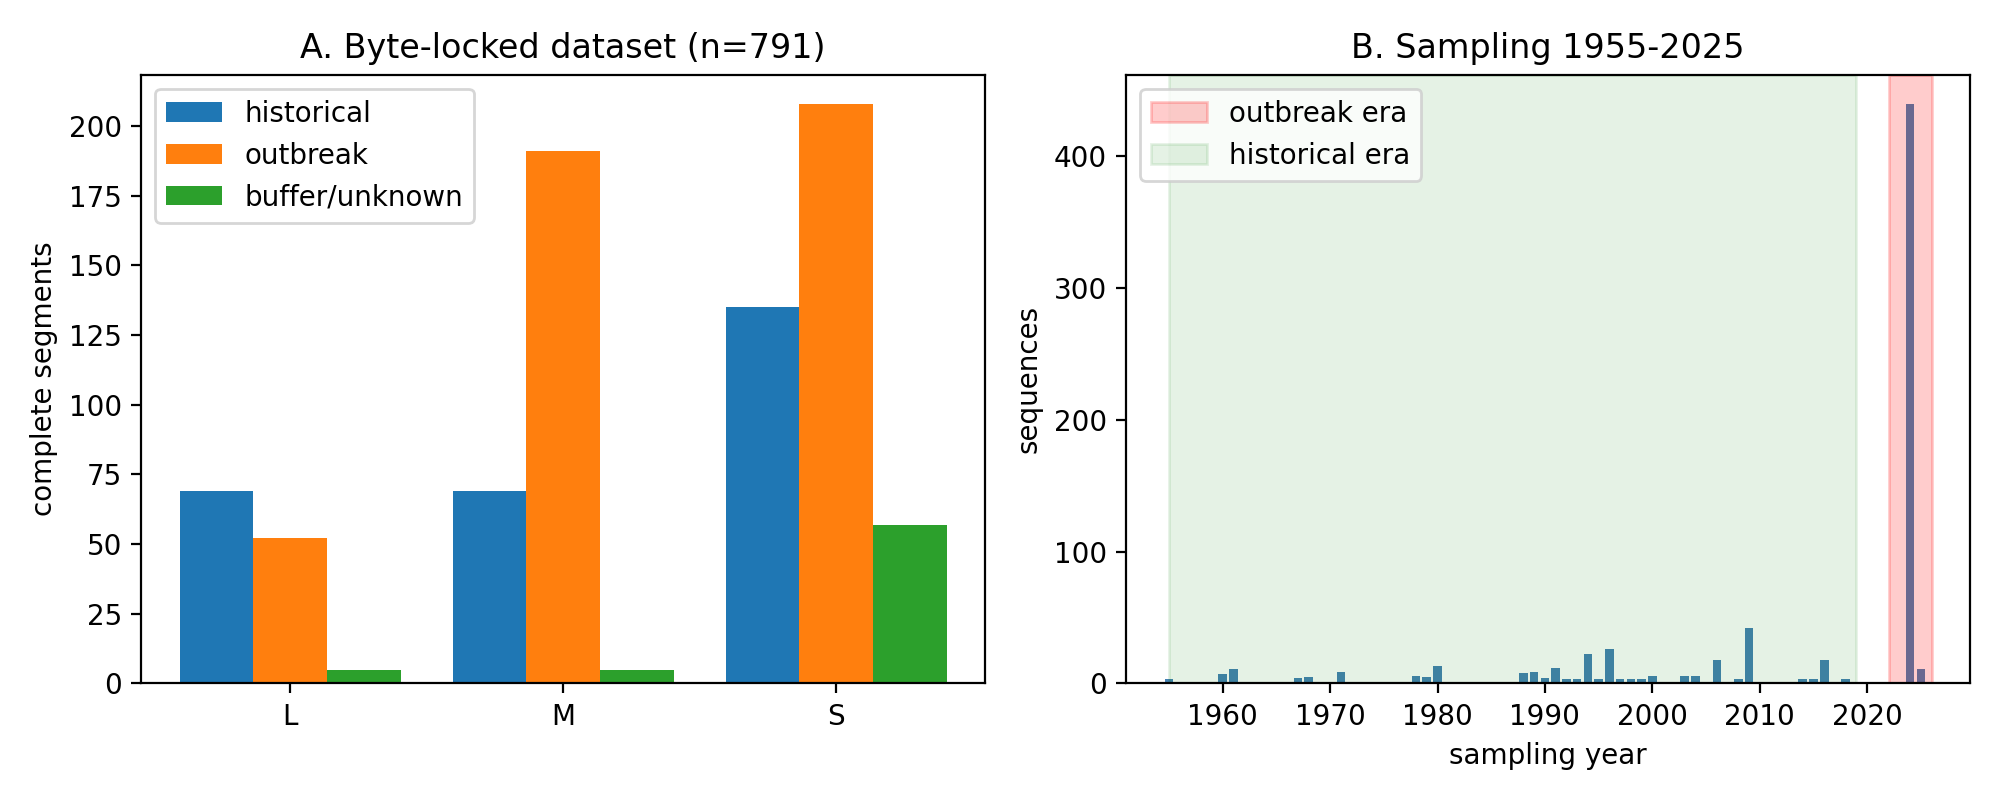
\includegraphics[width=\textwidth]{../figures/F1_dataset.png}
\caption{Byte-locked dataset. (A) Complete segments per segment and era. (B) Sampling-year distribution 1955--2025 with era windows.}\end{figure}
\begin{figure}[!htbp]\centering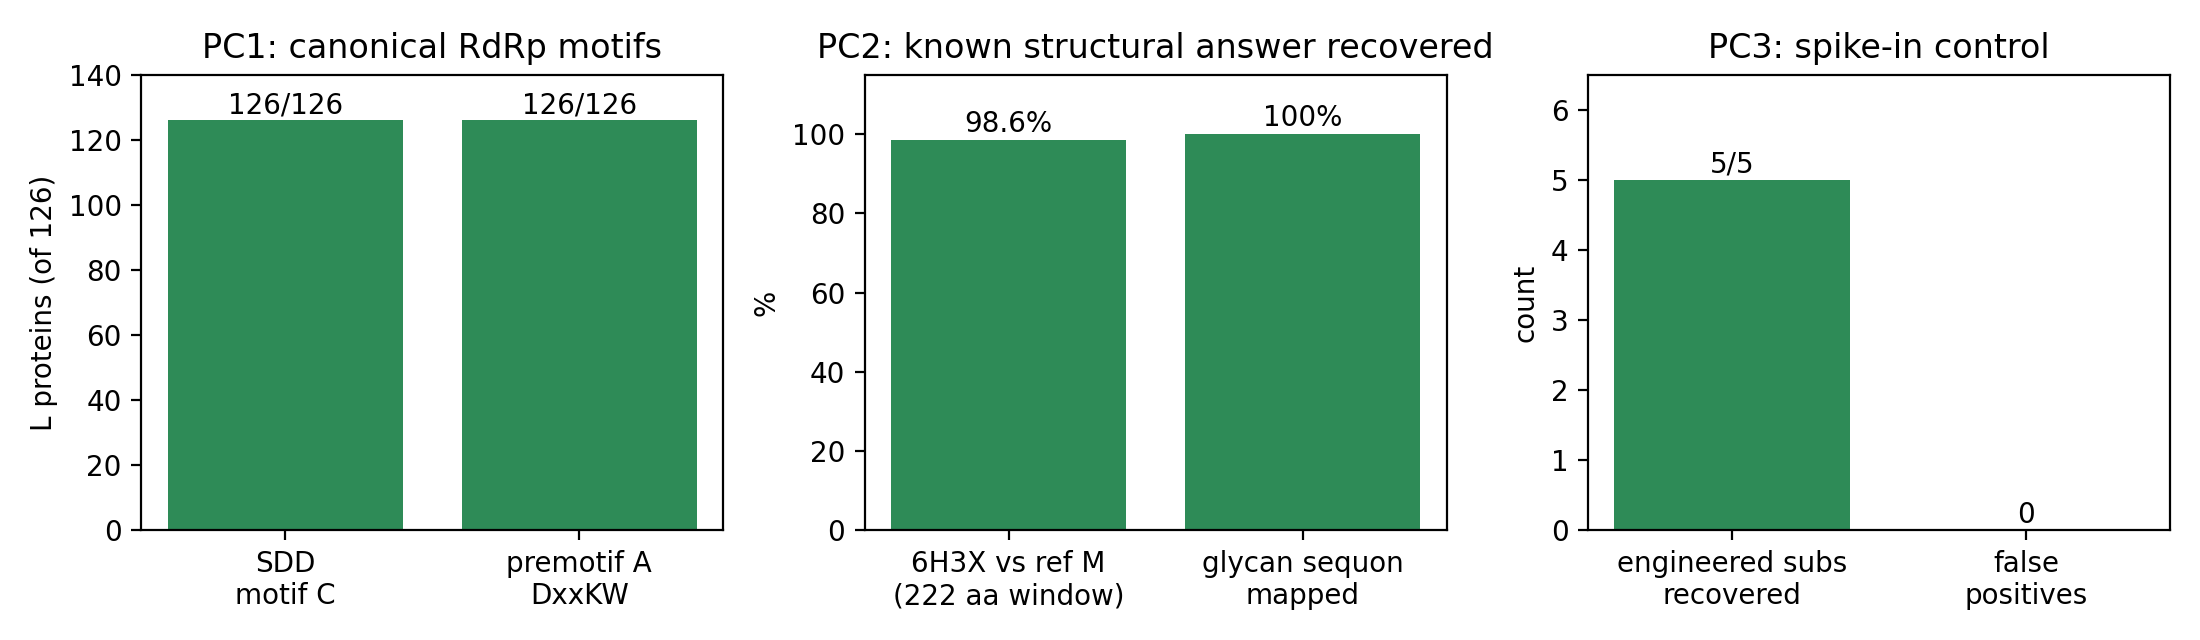
\includegraphics[width=\textwidth]{../figures/F2_validation.png}
\caption{Positive-control validations, all run before outbreak results were read.}\end{figure}
\begin{figure}[!htbp]\centering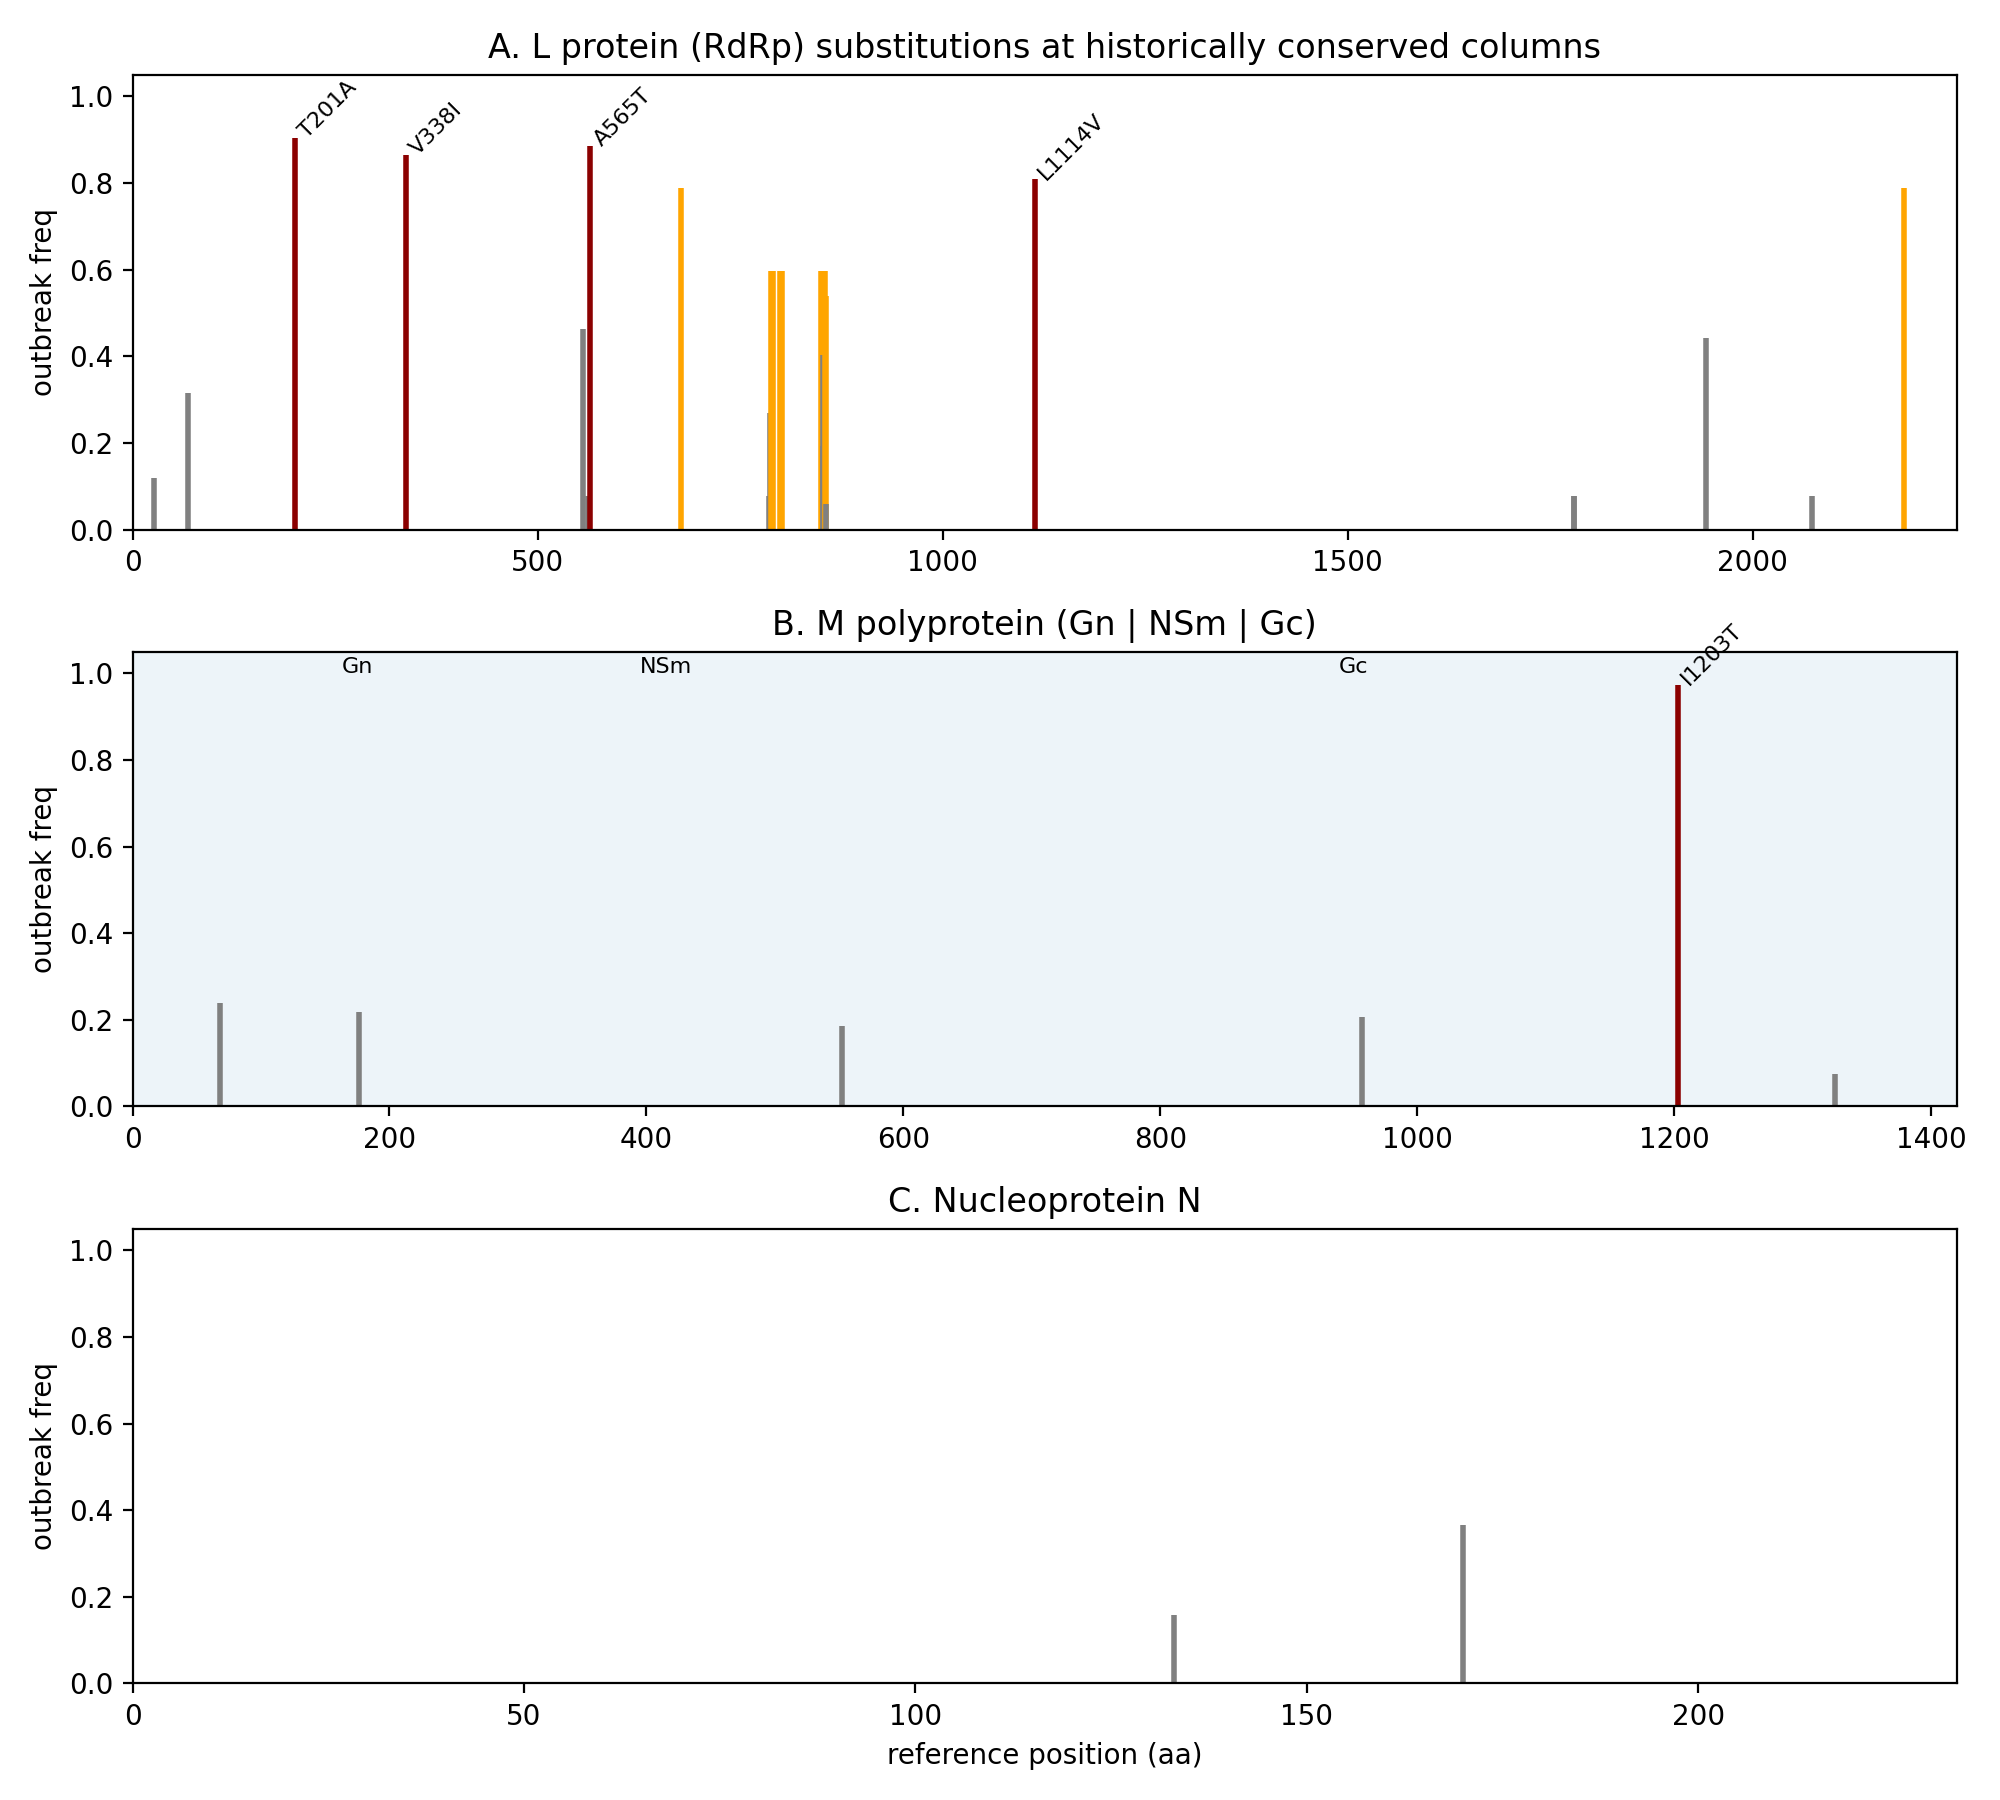
\includegraphics[width=\textwidth]{../figures/F3_substitutions.png}
\caption{Substitution catalog: outbreak frequency at historically conserved columns for L (A), M with Gn/NSm/Gc regions (B), and N (C). Sites $\geq$0.8 labeled.}\end{figure}
\begin{figure}[!htbp]\centering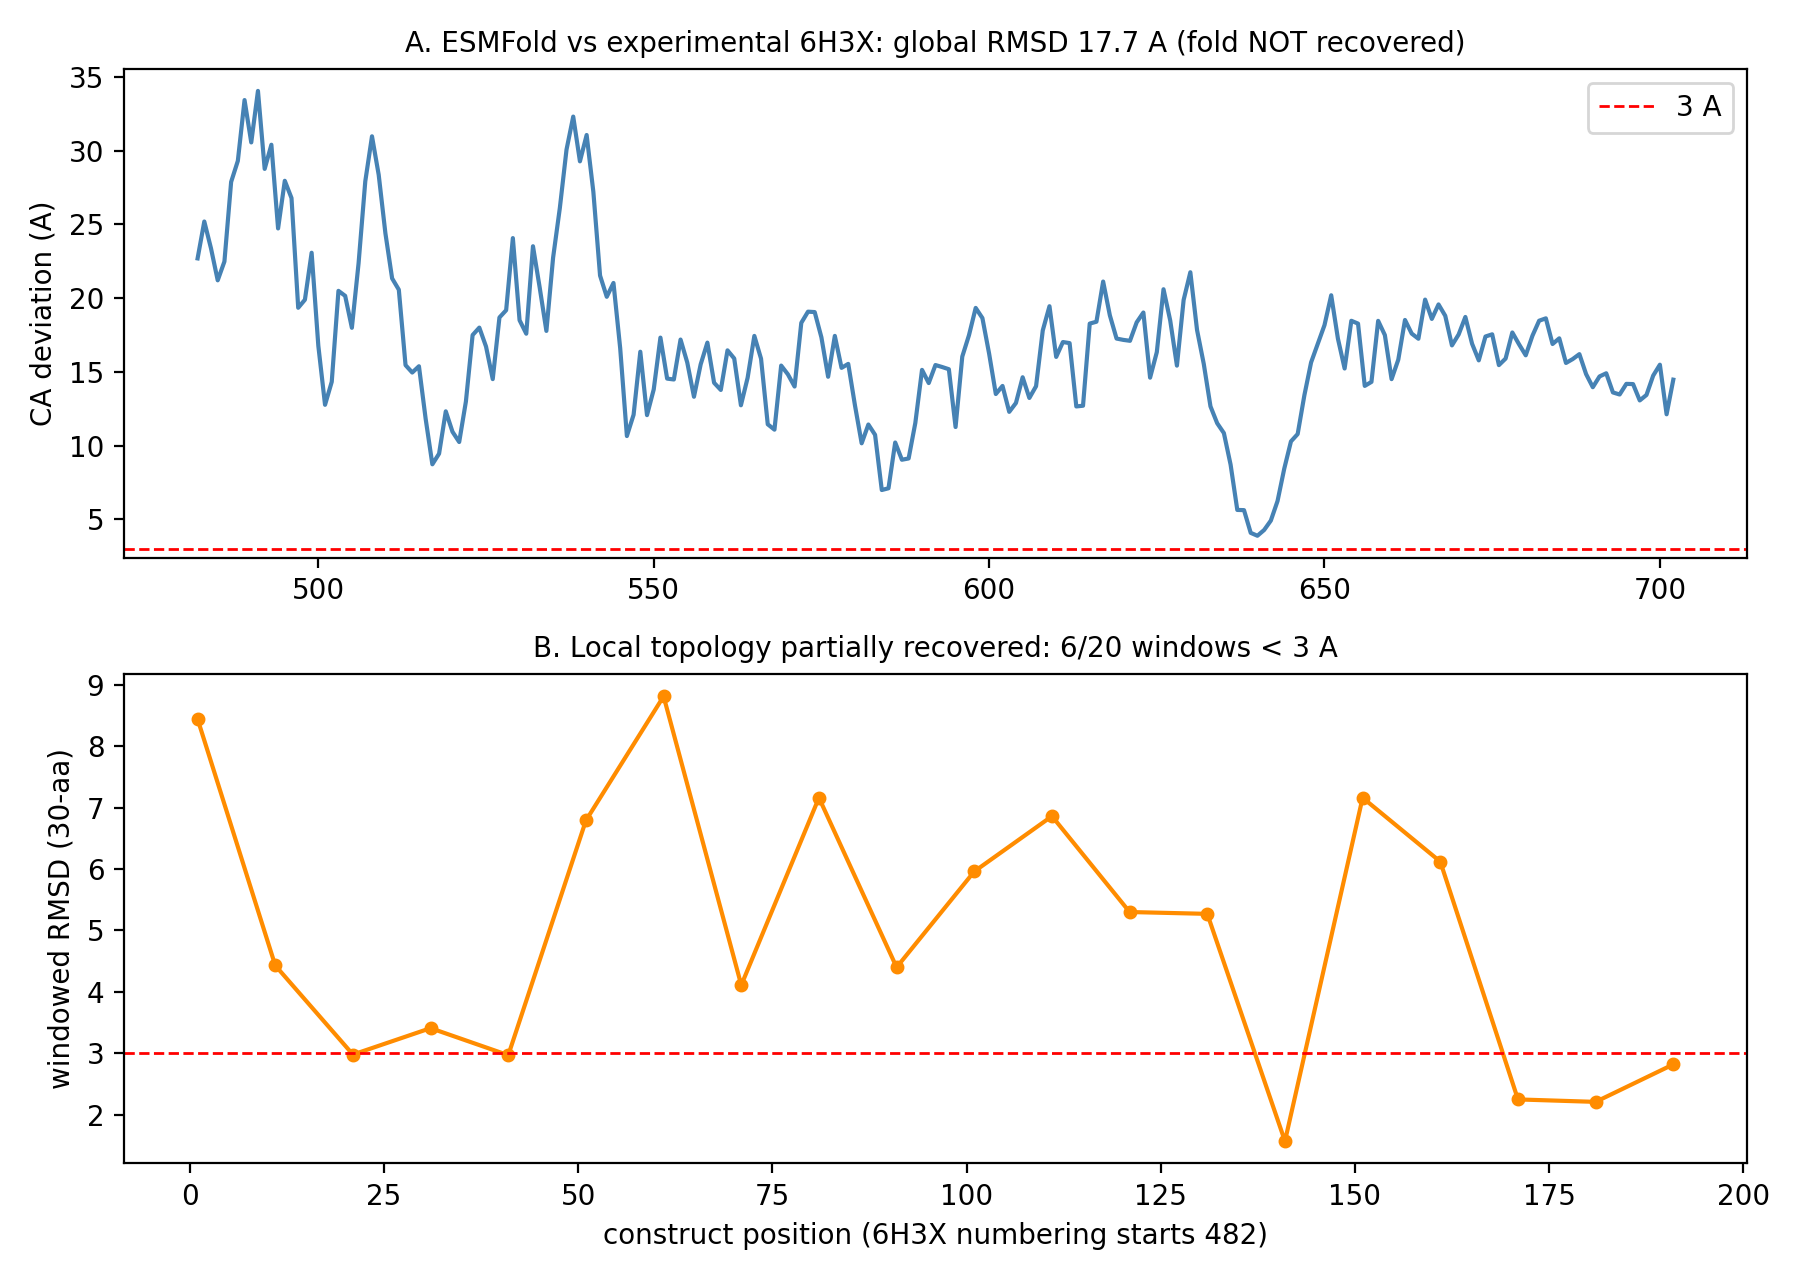
\includegraphics[width=0.9\textwidth]{../figures/F4_gchead_validation.png}
\caption{Structural positive control: ESMFold of the 6H3X construct vs experimental 6H3X. (A) Per-residue CA deviation after global superposition (RMSD 17.7 \AA{}). (B) 30-residue windowed RMSD; 6/20 windows $<$3 \AA{}.}\end{figure}
\begin{figure}[!htbp]\centering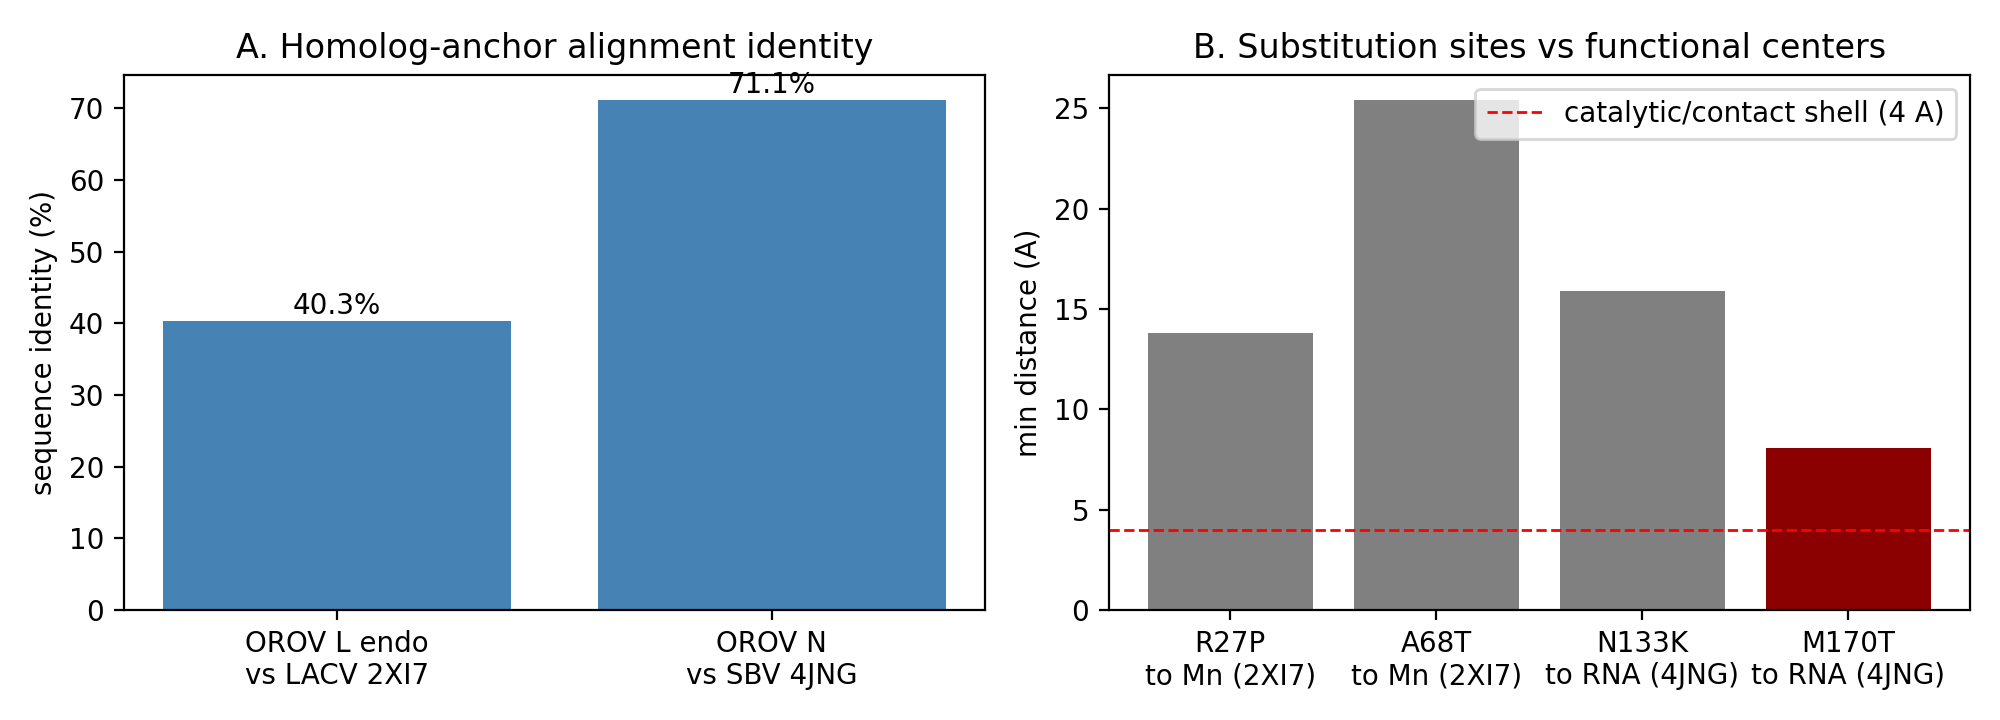
\includegraphics[width=\textwidth]{../figures/F5_homology.png}
\caption{Homolog anchors. (A) Alignment identity to experimental homologs. (B) Substitution-site distances to functional centers (2XI7 Mn$^{2+}$ ions; 4JNG RNA phosphate).}\end{figure}
\begin{figure}[!htbp]\centering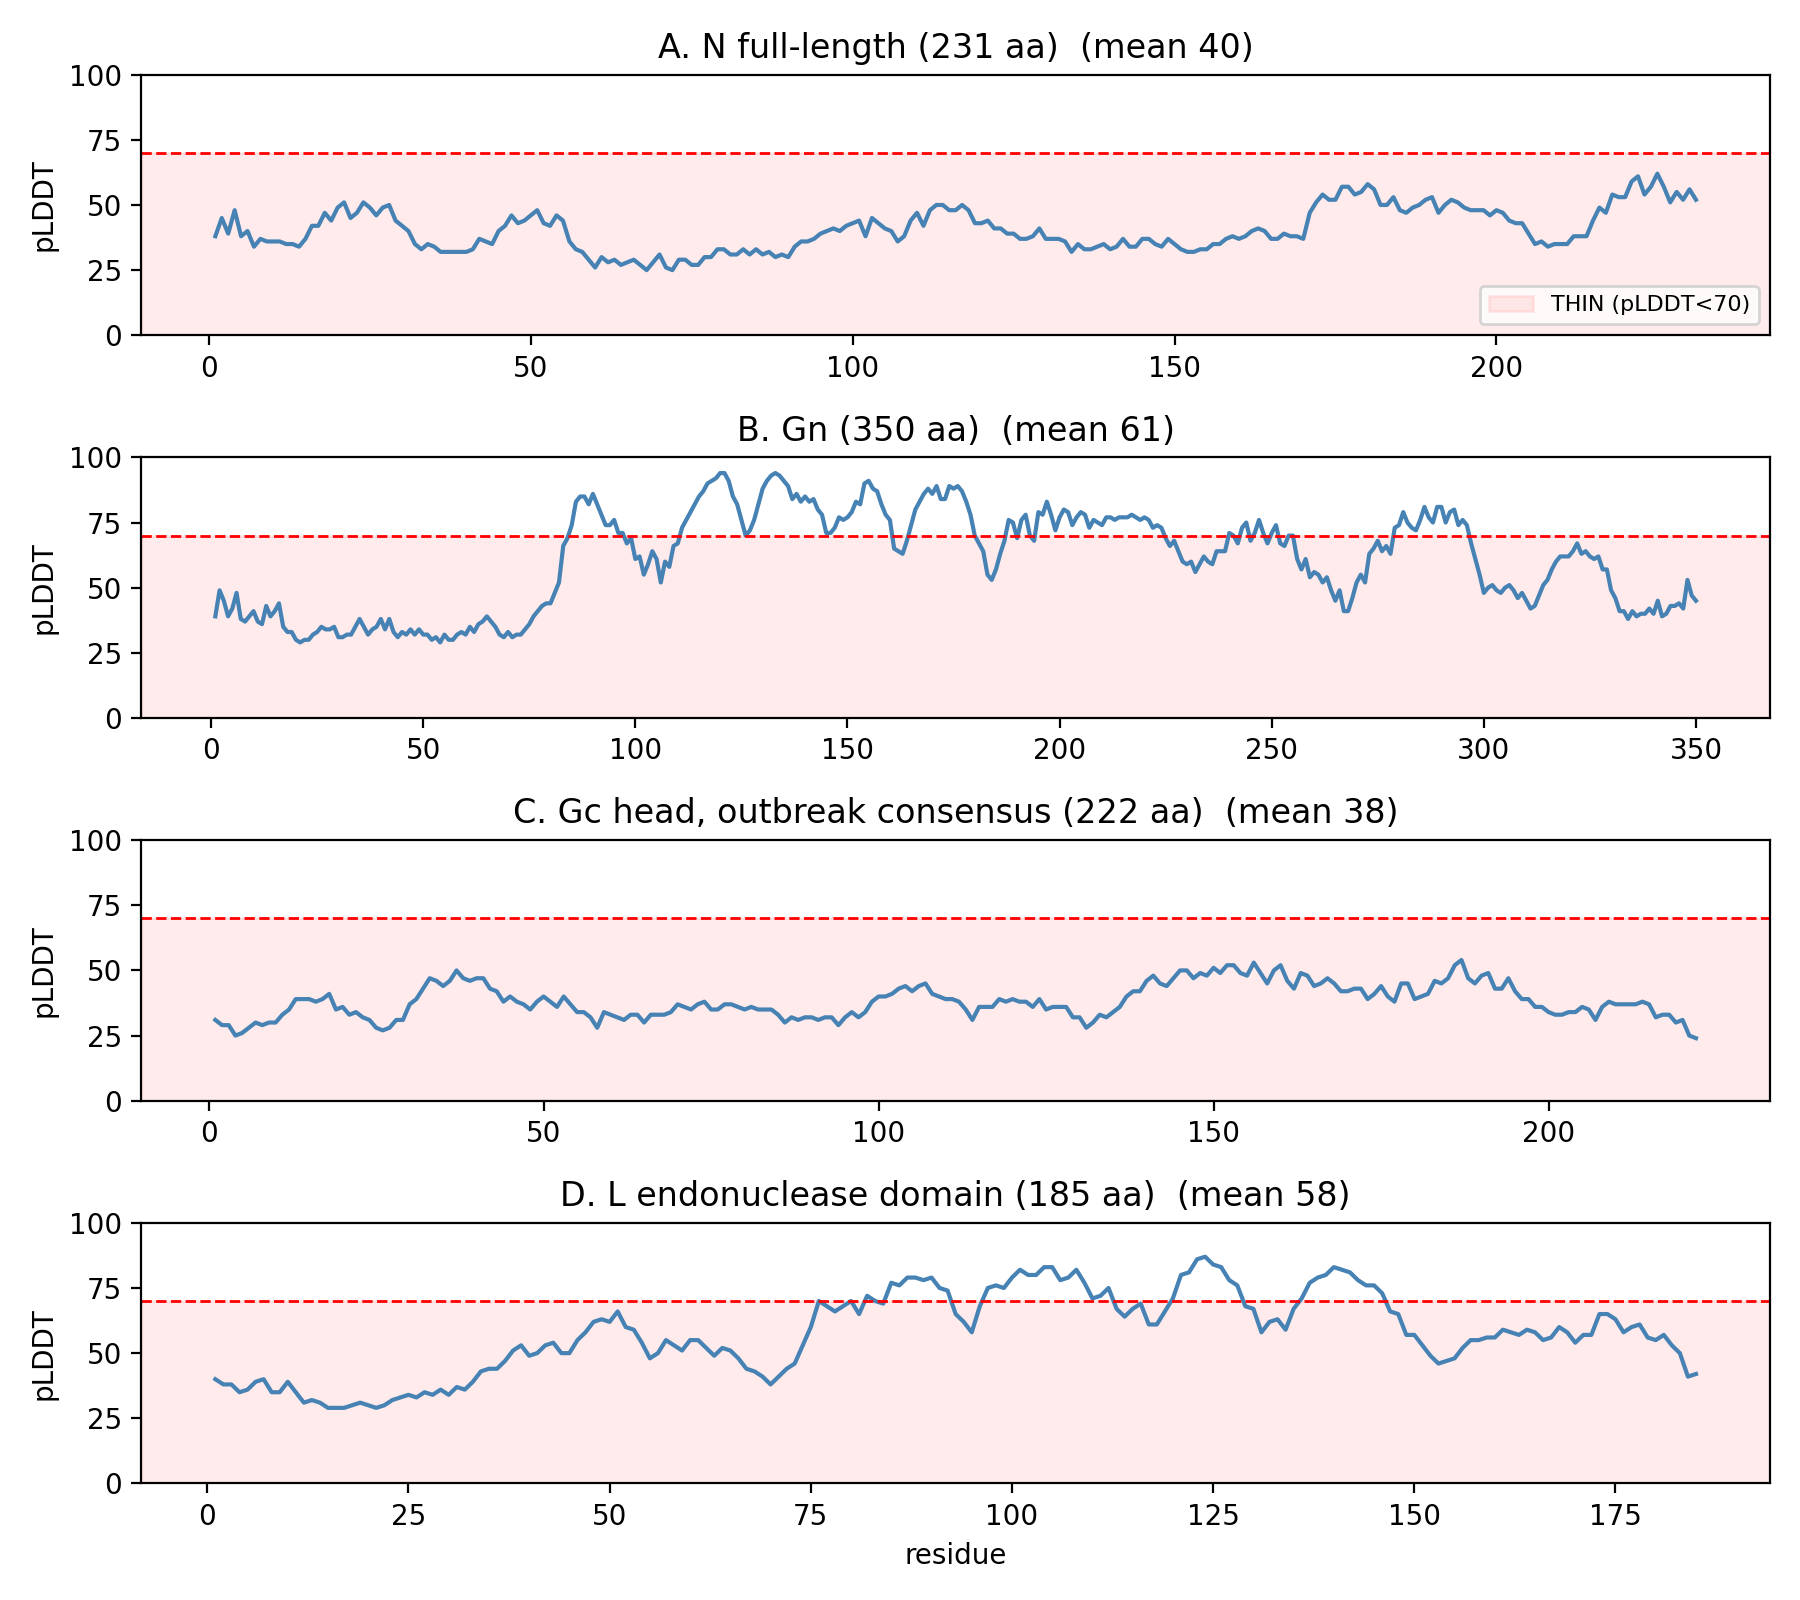
\includegraphics[width=0.85\textwidth]{../figures/F6_plddt.png}
\caption{Per-residue pLDDT (0--100) for the four ESMFold targets; red band marks THIN ($<$70). All four models are thin-dominated and support no claims per gate G2.}\end{figure}

\clearpage
\appendix
\section{Full substitution catalog}
\small
\begin{longtable}{llllrrrl}
\hline
Protein & Pos & Region & Hist AA (frac) & Alt AA & Out n & Out cov & Out frac \\
\hline
\endhead
L & 27 & L-endonuclease & R (1.0) & P & 6 & 51 & 0.118 \\
L & 68 & L-endonuclease & A (1.0) & T & 16 & 51 & 0.314 \\
L & 201 & L-other & T (1.0) & A & 47 & 52 & 0.904 \\
L & 338 & L-other & V (1.0) & I & 45 & 52 & 0.865 \\
L & 556 & L-other & A (1.0) & S & 24 & 52 & 0.462 \\
L & 562 & L-other & N (1.0) & S & 4 & 52 & 0.077 \\
L & 565 & L-other & A (0.986) & T & 46 & 52 & 0.885 \\
L & 677 & L-other & S (0.986) & A & 41 & 52 & 0.788 \\
L & 786 & L-polymerase-core & A (1.0) & V & 4 & 52 & 0.077 \\
L & 787 & L-polymerase-core & K (1.0) & N & 14 & 52 & 0.269 \\
L & 788 & L-polymerase-core & Q (1.0) & R & 31 & 52 & 0.596 \\
L & 790 & L-polymerase-core & V (1.0) & L & 31 & 52 & 0.596 \\
L & 791 & L-polymerase-core & N (1.0) & S & 31 & 52 & 0.596 \\
L & 799 & L-polymerase-core & I (1.0) & L & 31 & 52 & 0.596 \\
L & 802 & L-polymerase-core & N (1.0) & E & 31 & 52 & 0.596 \\
L & 850 & L-polymerase-core & K (1.0) & R & 31 & 52 & 0.596 \\
L & 853 & L-polymerase-core & T (1.0) & Q & 10 & 52 & 0.192 \\
L & 853 & L-polymerase-core & T (1.0) & L & 21 & 52 & 0.404 \\
L & 854 & L-polymerase-core & K (1.0) & R & 3 & 52 & 0.058 \\
L & 855 & L-polymerase-core & N (0.957) & M & 31 & 52 & 0.596 \\
L & 856 & L-polymerase-core & D (1.0) & M & 28 & 52 & 0.538 \\
L & 856 & L-polymerase-core & D (1.0) & I & 3 & 52 & 0.058 \\
L & 1114 & L-polymerase-core & L (1.0) & V & 42 & 52 & 0.808 \\
L & 1779 & L-other & I (1.0) & V & 4 & 52 & 0.077 \\
L & 1780 & L-other & E (1.0) & G & 4 & 52 & 0.077 \\
L & 1942 & L-other & V (0.986) & I & 23 & 52 & 0.442 \\
L & 2073 & L-other & D (1.0) & E & 4 & 52 & 0.077 \\
L & 2187 & L-other & I (0.986) & V & 41 & 52 & 0.788 \\
M & 68 & Gn & A (1.0) & T & 45 & 188 & 0.239 \\
M & 176 & Gn & V (0.986) & I & 41 & 188 & 0.218 \\
M & 552 & Gc & A (0.986) & S & 35 & 188 & 0.186 \\
M & 957 & Gc & I (0.971) & V & 39 & 188 & 0.207 \\
M & 1203 & Gc & I (1.0) & T & 183 & 188 & 0.973 \\
M & 1325 & Gc & P (1.0) & T & 14 & 188 & 0.074 \\
N & 133 & N & N (1.0) & K & 33 & 208 & 0.159 \\
N & 170 & N & M (1.0) & T & 76 & 208 & 0.365 \\
\hline
\end{longtable}
\normalsize
References: L ref KP026179.1, M ref KC759123.1, N ref HM470107.1. Positions are 1-based reference coordinates. Hist frac $=$ historical majority fraction; Out n/cov/frac $=$ outbreak carriers / coverage / frequency.

\section{Supplementary tables}
\subsection*{B.1 Geographic composition of the byte-locked dataset (top 12)}
\begin{center}\begin{tabular}{lr}
\hline
Country (as annotated) & Records \\
\hline
Brazil & 600 \\
unknown & 89 \\
Peru & 32 \\
Colombia & 18 \\
Ecuador & 18 \\
Panama & 13 \\
Italy & 6 \\
Trinidad and Tobago & 5 \\
Spain & 4 \\
Cuba & 3 \\
Haiti & 3 \\
\hline
All (incl. remainder) & 791 \\
\hline
\end{tabular}\end{center}
\subsection*{B.2 Validation run log}
\begin{center}\begin{tabular}{lll}
\hline
Control & Result & Detail \\
\hline
PC1 RdRp motifs & PASS & SDD 126/126; DxxKW 126/126 \\
PC2 6H3X sequon & PASS & 98.6\% identity; NIT sequon at ref 676 \\
PC3 spike-in, run 1 & FAIL (logged) & baseline-vs-majority design flaw; control corrected \\
PC3 spike-in, run 2 & PASS & 5/5 recovered, 0 false positives \\
G3 re-run reproducibility & PASS & substitutions.tsv byte-identical (diff-verified) \\
Structural PC (ESMFold vs 6H3X) & FAIL (preserved) & global CA RMSD 17.7 \AA{}; claims restricted \\
\hline
\end{tabular}\end{center}

\section{Reproducibility README}
\textbf{Restore procedure.} (1) Re-fetch accessions listed in \texttt{data/manifest.tsv} from NCBI E-utilities; verify each record against its per-record SHA-256 and the set-level checksums in \texttt{data/BYTELOCK.txt}. (2) \texttt{python3 code/extract\_cds.py} regenerates protein sets from GenBank CDS annotations. (3) \texttt{python3 code/mutation\_pipeline.py} re-runs PC3 (refuses to emit results on failure), then writes \texttt{results/substitutions.tsv}; the run is byte-identical (diff-verified 2026-09-23). (4) \texttt{code/make\_consensus.py} rebuilds structure targets; ESMFold calls and 6H3X/2XI7/4JNG downloads regenerate structure products; validation scripts reproduce \texttt{results/gc\_head\_validation.csv} and \texttt{results/gc\_head\_windowed\_rmsd.csv}. Environment: python 3.10, biopython 1.88, parasail 1.3.4, pandas, numpy, matplotlib; network access to NCBI, RCSB, ESM Atlas. No GPU required; runtime $\sim$5 minutes excluding network.

\section{Byte-lock record}
Set-level SHA-256 (locked 2026-09-23 13:29 IST):\\
\texttt{orov\_L\_complete.fasta} ebadf3e1b7dc645ae167a4f898cdf4c9e4da11704c6a4e0f4e024b5f70c9440b\\
\texttt{orov\_M\_complete.fasta} 82cd04d0b8998eb4e2db4fb984459873b084e50d6a61ac99f46be6f10709a7f2\\
\texttt{orov\_S\_complete.fasta} fd8d7c41f526cf362ab6c2b1ce8c58f685a83198ec7bc224be18f89a83e4f503\\
\texttt{manifest.tsv} ca4ea79c04968d058062e06a478156635220f39bb5e2f5a5dcdd7de9690dca6b\\
Per-record checksums: \texttt{data/manifest.tsv} (791 rows).
\end{document}
